% +--------------------------------------------------------------------+
% | Sample Chapter
% |
% | This file provides examples of how to
% | - insert a figure with a caption
% | - construct a table with a caption
% | - create subsections within the chapter
% | - insert a reference to a Figure or Table
% | - make a citation
% +--------------------------------------------------------------------+

\cleardoublepage

% +--------------------------------------------------------------------+
% | Replace "Chapter Title" below with the title of your chapter.  LaTeX
% | will automatically number the chapters.
% +--------------------------------------------------------------------+

\chapter{Introducción}
%\label{ch:chapter1}
\label{makereference}

Entre los años 2008 y 2009 comenzaron a usar el concepto Internet de las cosas (abreviado IoT) como una apuesta hacia el futuro, cuyo objetivo era interconectar dispositivos digitales a internet.

Esto ya es una realidad, con mayor frecuencia encontramos nuevos dispositivos capaces de conectarse a internet, permitiendo al usuario su manejo desde cualquier parte del mundo. Con ello se abre camino a nuevas oportunidades haciendo la vida más cómoda al usuario y proporcionándole mayor seguridad y control.

Según empresas del sector tecnológico, en 2016 se espera que haya más  de 6.000 millones de dispositivos basados en este concepto.

El concepto del internet de las cosas agrupa múltiples capacidades, algunas de ellas han sido utilizadas en el proyecto, estas se nombran a continuación:

\textbf{Comunicación y cooperación:} Dispositivos capaces de conectarse a la red de internet y entre ellos, intercambiando datos y comunicándose con servidores.

\textbf{Direccionamiento:} Los objetos serán localizables y configurables desde cualquier lugar de la red de internet.

\textbf{Identificación:} Los objetos se identificarán en la red por medio de tecnologías como RFID (Radio Frecuency Identification), códigos de barras ópticos, NFC (Near Field Communication) y otras muchas formas.

\textbf{Localización:} Se podrá saber la ubicación física del dispositivo en cualquier momento.

El proyecto nace con el objetivo de emprender en esta tecnología, para ello se quiere conectar entre sí un sensor de acelerometría y un microprocesador para recibir y procesar sus datos. Dicho microprocesador debe estar provisto de Bluetooth de bajo consumo (en inglés, Bluetooth Low Energy o BLE) para poder enviar los datos vía Bluetooth a una aplicación móvil desarrollada en Android creada por los alumnos.

Existe una amplia variedad de dispositivos de bajo coste que podrían considerarse, ya que el mercado de los microprocesadores de bajo consumo está ahora en expansión y hay gran oferta de estos dispositivos, con entornos de desarrollo que ofrecen distintas alternativas y que previsiblemente irán reduciéndose en los próximos años cuando predomine una tecnología que se imponga a las demás.

Unas de las  empresas más especializadas en este tipo de tecnologías y que resaltan en este mercado son \textbf{Nordic Semiconductor, Cypress Semiconductor, Texas Instruments (TI), Cambridge Silicon Radio (CSR)} y \textbf{Dialog Semiconductor}.

Destacamos 2 empresas que nos han ofrecido mejores soluciones de microprocesadores de bajo consumo según las necesidades del proyecto:

\textbf{Nordic} está a la vanguardia de la revolución inalámbrica y son especialistas en Radiofrecuencia de consumo ultra bajo (ULP) redefiniendo nuevos procesadores por su bajo consumo, precios competitivos y aumentando la potencia de estos.
La empresa de semiconductores integra procesadores basados en la arquitectura ARM de 32 y 64 bits que predominan en el mercado de la electrónica. Son procesadores relativamente simples siendo ideales para aplicaciones de bajo consumo y tiene un precio económico. 

\textbf{Cypress} es una empresa especializada en ofrecer soluciones de alta calidad para sistemas integrados en el sector aeroespacial, automoción, industria, redes, telecomunicaciones y electrónica de consumo, entre otros campos. Cubre una amplia gama de productos entre los cuales destacan los microprocesadores, memorias,  sistemas programables en chips , lo que denominan (en inglés Programable System on Chip o PSOC), controladores táctiles capacitivos y controladores inalámbricos Bluetooth de bajo consumo

\section{Entornos de desarrollo}
\label{makereference1.1}

Con los dispositivos de bajo consumo nacen también multitud de entornos de desarrollo específicos para desarrollar todo su potencial, lo que dificulta la exploración de hardware, pues es necesario trabajar con un nuevo entorno cada vez. 

mbed, creada por la empresa ARM, es una plataforma de desarrollo \textit{online} que intenta hacer frente a esta variedad de entornos facilitando el desarrollo de prototipos de sistemas basados en microprocesadores.

Esta plataforma se creó para promover el Internet de las Cosas (IoT) y desarrollar proyectos mediante herramientas de construcción de hardware y software que aceleren el desarrollo de dispositivos basados en ARM.

Su enfoque está basado en la \textit{nube} y permite codificar, añadir librerías y compilar desde un navegador web. La ventaja de programar desde cualquier navegador es que permite tener accesibilidad desde cualquier punto del mundo sólo con conexión a internet. Durante el Capítulo~\ref{makereference4} se explicará con más detalle este entorno y cómo nos ha ayudado a llevar a cabo este proyecto.

La placa de desarrollo que se ha utilizado, la nRF51-DK de Nordic, que utiliza el SoC BLE nRF51822, es compatible con mbed.

\section{Bluetooth Smart: Bluetooth de bajo consumo}
\label{makereference1.2}

Uno de los rasgos fundamentales de IoT es la conectividad.

Lo que conocíamos como Bluetooth 4.0 ha cambiado de nombre y mejorado notablemente sus características. Usa poca energía de consumo y latencia y funciona con dispositivos en un rango corto de hasta 50 metros. De ahora en adelante se conocerá como la versión inteligente, es decir, Bluetooth Smart. 
Sus características lo hacen perfecto para dispositivos que necesitan funcionar con una batería pequeña durante largos períodos.

\section{Especificación del objetivo del proyecto}
\label{makereference1.3}

El proyecto consiste en medir valores de acelerometría por medio de un sensor y conectado a través de Bluetooth Smart a un dispositivo móvil para posteriormente poder analizar los datos reproducidos desde una aplicación móvil creada en Android.
La medición se hará durante un recorrido determinado por el usuario y utilizando el GPS de su dispositivo móvil Android,podrá visualizar el recorrido realizado observando la aceleración que realizó así como otros datos de interés del recorrido del usuario.
El medio de transporte utilizado será una bicicleta y el dispositivo irá sujeto y fijado al cuadro de la misma.

%\begin{figure}[htb]%t=top, b=bottom, h=here
%
%    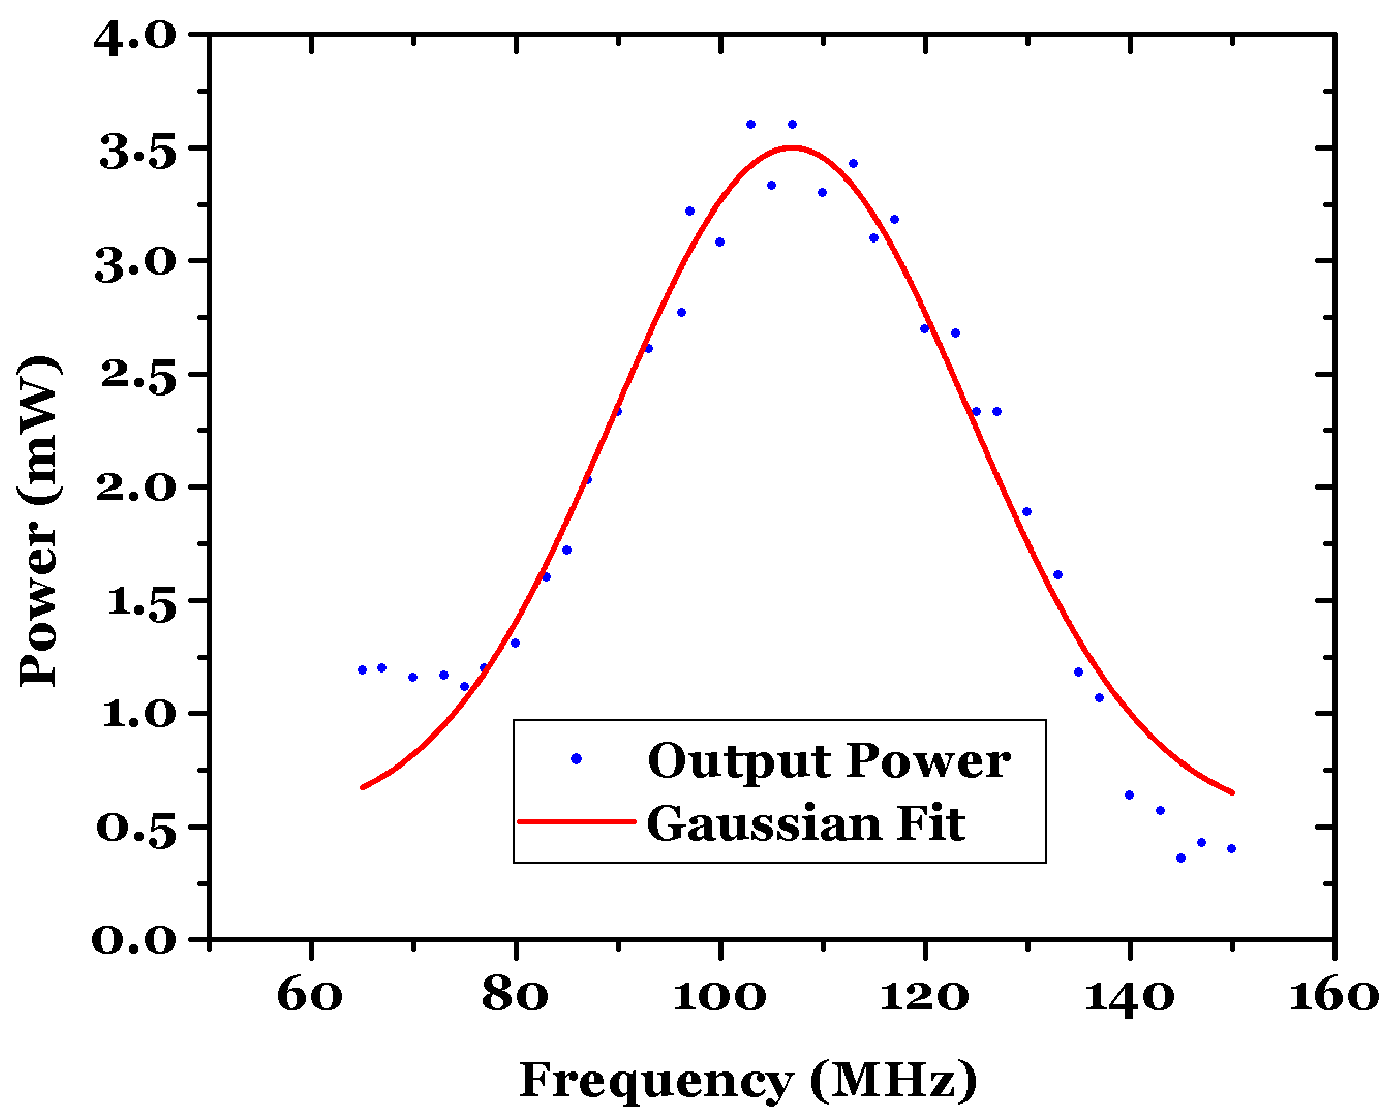
\includegraphics[height=2.5in]{figures/graph.png}
%
%    \caption[Optional: Short caption to appear in List of
%    Figures]{Full caption to appear below the Figure}
%
%   \label{figure1}
%\end{figure}

% +--------------------------------------------------------------------+
% |To create cross-references to figures, tables and segments
% |of text, LaTeX provides the following commands:
% |   \label{marker}
% |   \ref{marker}
% |   \pageref{marker}
% | where {marker} is a unique identifier.
% |
% | In the line above, we use \label{figure1} to mark a location
% | we wish to refer to later.  LATEX replaces \ref by the number of
% | the chapter, section, subsection, figure, or table after which the
% | corresponding \label command was issued. \pageref prints the page
% | number of the page where the \label command occurred.
% |
% +--------------------------------------------------------------------+

%Here is an example of a Table:

%\begin{table}

% +--------------------------------------------------------------------+
% | We include the command \begin{center} to center the table
% | horizontally on the page.  Note use of the command \end{center}
% | to turn off centering after the table is defined.
% +--------------------------------------------------------------------+
%    \begin{center}

% +--------------------------------------------------------------------+
% | The table is created with this command
% |
% | \begin{tabular}[pos]{table spec}
% |
% | The "pos" argument specifies the vertical position of the table relative to
% | the baseline of the surrounding text.  Use t, b, or c to specify alignment
% | at the top, bottom, or center.
% |
% | The "table spec" command defines the format of the table
% |   l for a column of left-aligned text
% |   r for a column of right-aligned text
% |   c for centered text
% |   p{width} for a column containing justified text with line breaks
% |   | for a vertical line
% +--------------------------------------------------------------------+

%    \begin{tabular}[c]{|c|c|c|}
%        \hline
%        Column 1 Heading & Column 2 Heading & Column 3 Heading \\
%        \hline
%        Col 1 Row 1 & Col 2 Row 1 & Col 3 Row 1\\
%        Col 1 Row 2 & Col 2 Row 2 & Col 3 Row 2\\
%        Col 1 Row 3 & Col 2 Row 3 & Col 3 Row 3\\
%        \hline
%    \end{tabular}
%    \caption{Caption to appear below the table}
%    \label{table1}
%   \end{center}
%\end{table}

% +--------------------------------------------------------------------+
% | Replace \section headings below with the title of your
% | subsections.  LaTeX will automatically number the subsections 1.1,
% | 1.2, 1.3, etc.
% +--------------------------------------------------------------------+

%In this paragraph, we want to refer to Fig.~\ref{figure1}
%mentioned at the beginning of this chapter.  We also refer to the
%Table~\ref{table1}.

%\section{Making a Reference to a Chapter Subsection}
%\label{makereference1.2}

%In this section, we refer back to text mentioned in
%Section~\ref{makereference1.1} on page~\pageref{makereference1.1}.

%\section{Making a Citation}
%\label{makereference1.3}

%Here's an example of a citation to a single
%work.~\citet{CT:Weiner:1999} It's also possible to make multiple
%citations.~\citet{CT:Phillips:1985, ARP:Loy:1974}
